\documentclass[11pt,a4paper]{article}
\usepackage[T1]{fontenc}
\usepackage[margin=2.3cm]{geometry}
\usepackage{amsmath,amssymb}
\usepackage{graphicx}
\usepackage[dvipsnames]{xcolor}
\usepackage{enumitem}
\usepackage[colorlinks=true,linkcolor=blue,urlcolor=blue]{hyperref}
\setlength{\parskip}{0.6em}
\setlength{\parindent}{0pt}
\begin{document}

\begin{center}{\LARGE\bfseries opensculpt}\\[0.4em]{\large Model a mug and other CAD parts as distance functions, in three sessions.}\\[0.2em]\small PAN IIT OSS explainer \textbullet{} diploma / undergraduate to advanced undergraduate (levels 5-6)\end{center}

\section*{Why this exists}
A CAD part can be stored as a function that says how far every point of space is from its surface. This explainer shows how simple operations on such functions (min, max, smooth blends) build real parts, and how to measure them on a grid.

\section*{The end goal}
Model a mug and other CAD parts with signed distance functions. The end goal is to model a mug and other CAD parts with signed distance functions, as used in modern geometry kernels and GUI tools: a parametric part whose length, hole and wall change while its volume and drawing update.

\section*{How the three sessions build up}
\begin{enumerate}[nosep]
\item \textbf{Session 1: A shape is a function: signed distance} (Level 1, conceptual interactive model, 60 min).
\item \textbf{Session 2: CAD operations on distance functions: a parametric mug} (Level 2, mathematical engineering model, 75 min).
\item \textbf{Session 3: A 3D mug on a voxel grid: measure it and check it} (Level 3, simulation and validation, 90 min).
\end{enumerate}

\section{Session 1: A shape is a function: signed distance}

\subsection*{A. Real-world problem}
A CAD program holds a mug and must answer, millions of times per second, one question: is this point inside the mug? Instead of storing a list of faces, we can store a function: give it any point and it returns one number, the distance to the nearest surface, with a minus sign if the point is inside. Can you describe a circle and a box that way, draw them as pictures, and use the numbers to join the shapes?

\subsection*{B. Concept and theory}
Take a point p = (x, y). For a circle with centre c and radius r, the signed distance is \textbar{}p - c\textbar{} - r: positive outside, zero on the edge, negative inside, and -r at the centre. For a box with centre c and half-sizes (a, b), first compute q = \textbar{}p - c\textbar{} - (a, b) separately for x and y. If both parts of q are negative the point is inside and the distance to the nearest side is the larger part of q (the one closest to zero). Otherwise the distance is the length of the vector made of the positive parts of q. The shape itself is the set of points where the value is negative; its surface is where the value is zero. A point in the union of two shapes is inside at least one of them, so the union has value min(d1, d2). A true signed distance cannot change faster than you move: a step of length s changes it by at most s.

\begin{itemize}[nosep]
\item p = (x, y): a point in the plane (units (any length unit))
\item c: centre of a circle or box (units)
\item r: radius of the circle (units)
\item (a, b): half-width and half-height of the box (units)
\item d: signed distance (negative inside) (units)
\end{itemize}

\begin{equation*}
d_{\text{circle}}(\mathbf p)=|\mathbf p-\mathbf c|-r
\end{equation*}

\begin{equation*}
\mathbf q=\big(|x-c_x|-a,\ |y-c_y|-b\big),\qquad d_{\text{box}}(\mathbf p)=\big|\max(\mathbf q,\mathbf 0)\big|+\min\big(\max(q_x,q_y),0\big)
\end{equation*}

\begin{equation*}
d_{\text{union}}=\min(d_1,\ d_2)
\end{equation*}

\begin{center}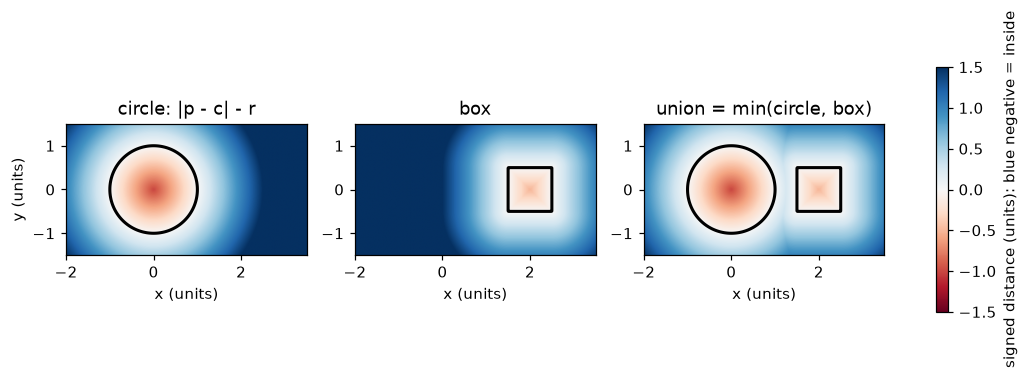
\includegraphics[width=0.85\linewidth]{figures/s01_sdf_pictures.png}\\\small Circle, box and union as colour fields; the black line is the surface (value 0).\end{center}

\subsection*{E. Worked example}
A circle has radius 1 and centre (0, 0). A box has centre (2, 0) and half-sizes (0.5, 0.5). Find the signed distance of the point (1.2, 0.3) to each shape and to their union.
\begin{enumerate}[nosep]
\item Circle: \textbar{}p - c\textbar{} = sqrt(1.2\textasciicircum{}2 + 0.3\textasciicircum{}2) = sqrt(1.53) = 1.237, so d = 1.237 - 1 = 0.237.
\item Box: q = (\textbar{}1.2 - 2\textbar{} - 0.5, \textbar{}0.3 - 0\textbar{} - 0.5) = (0.3, -0.2).
\item The positive parts of q are (0.3, 0), of length 0.3, and max(qx, qy) = 0.3 is not negative, so the inside term is 0 and d = 0.3.
\item Union = min(0.237, 0.300) = 0.237. The value is positive, so the point is outside both shapes, closest to the circle.
\end{enumerate}
\textbf{Answer.} Circle 0.237, box 0.300, union 0.237 (all in the same unit as the coordinates): the point is outside.

\subsection*{F. Questions}
\begin{enumerate}[nosep]
\item \textbf{Conceptual.} Why do we use a negative value for points inside a shape, rather than just the distance to the surface?
\item \textbf{Numerical.} A circle of radius 2 is centred at the origin. What is the signed distance of the point (3, 4)? Is it inside?
\item \textbf{Graph and simulation interpretation.} In the profile graph along the line y = 0.3, between which x values is the union inside? Why are there two separate stretches?
\item \textbf{Design and optimisation challenge.} Design: the box has centre (2, 0) and half-sizes (0.5, 0.5). Choose the radius of a circle centred at the origin so that the two shapes just touch, then so that they overlap. Which is better for a real part and why?
\end{enumerate}

\section{Session 2: CAD operations on distance functions: a parametric mug}

\subsection*{A. Real-world problem}
A designer needs a mug that holds 300 mL. The height is fixed at 9 cm by the shelf; the wall thickness and the radius are free. How do we build the mug from simple shapes, let a program change its size, and compute its volume and capacity? Lengths are in cm, so 1 cm\textasciicircum{}3 = 1 mL.

\subsection*{B. Concept and theory}
With signed distances a and b: intersection is max(a, b) (inside both), subtraction a minus b is max(a, -b) (inside a and not inside b), an offset that grows a shape by t is a - t, and a shell of thickness t on each side of the surface is \textbar{}a\textbar{} - t. Plain min leaves a sharp crease where two shapes meet; a smooth minimum rounds it. With blend radius k we use h = max(k - \textbar{}a - b\textbar{}, 0) / k and smin = min(a, b) - h\textasciicircum{}2 k / 4. When \textbar{}a - b\textbar{} \textgreater{}= k, h = 0 and smin equals min exactly; when a = b the surface is pulled outward by the largest amount, k / 4. The mug cross-section lives in the plane (x, z): the outer wall is a box of half-width R from z = 0 to z = H, the cavity is a box of half-width R - t that starts at the floor z = t and rises above the rim, and the handle is a ring \textbar{}circle\textbar{} - tube radius, clipped to stay outside the cavity and blended to the body. Because the body is a solid of revolution about the axis, its capacity is pi (R - t)\textasciicircum{}2 (H - t) and its material is pi R\textasciicircum{}2 H minus the capacity; solving for the radius gives R = t + sqrt(V / (pi (H - t))).

\begin{itemize}[nosep]
\item R: outer radius of the mug (cm)
\item H: height of the mug (cm)
\item t: wall and floor thickness (cm)
\item k: blend radius of the smooth union (cm)
\item V: capacity (volume the mug holds) (mL = cm\textasciicircum{}3)
\item a, b: signed distances of two shapes (cm)
\end{itemize}

\begin{equation*}
d_{\cap}=\max(a,b),\qquad d_{A\setminus B}=\max(a,-b),\qquad d_{\text{shell}}=|a|-t
\end{equation*}

\begin{equation*}
h=\frac{\max(k-|a-b|,\,0)}{k},\qquad \mathrm{smin}(a,b)=\min(a,b)-\frac{k\,h^{2}}{4}
\end{equation*}

\begin{equation*}
V_{\text{cavity}}=\pi\,(R-t)^{2}(H-t),\qquad V_{\text{material}}=\pi R^{2}H-V_{\text{cavity}}
\end{equation*}

\begin{equation*}
R=t+\sqrt{\dfrac{V}{\pi\,(H-t)}}
\end{equation*}

\begin{center}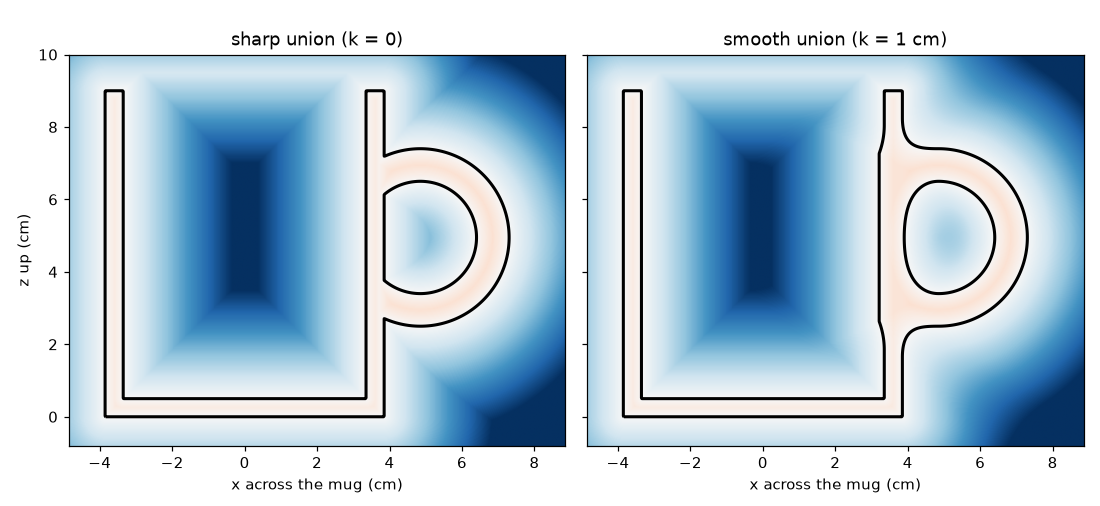
\includegraphics[width=0.85\linewidth]{figures/s02_mug_section.png}\\\small The mug cross-section from signed distances: sharp union (left) and smooth union with blend 1 cm (right).\end{center}

\subsection*{E. Worked example}
Find the outer radius of a mug of height 9 cm and wall 0.5 cm that holds exactly 300 mL, and the volume of material in the body.
\begin{enumerate}[nosep]
\item Capacity = pi (R - t)\textasciicircum{}2 (H - t), with H - t = 9 - 0.5 = 8.5 cm.
\item (R - t)\textasciicircum{}2 = 300 / (pi * 8.5) = 11.23, so R - t = 3.352 cm.
\item R = 0.5 + 3.352 = 3.852 cm.
\item Material = pi R\textasciicircum{}2 H - 300 = pi * 3.852\textasciicircum{}2 * 9 - 300 = 419.5 - 300 = 119.5 cm\textasciicircum{}3.
\end{enumerate}
\textbf{Answer.} R = 3.852 cm; the body holds 300 mL and contains 119.5 cm\textasciicircum{}3 of material.

\subsection*{F. Questions}
\begin{enumerate}[nosep]
\item \textbf{Conceptual.} Why does the smooth union add material only near the place where the two shapes come close, and not everywhere?
\item \textbf{Numerical.} Find the outer radius for a mug of height 10 cm and wall 0.4 cm that holds 300 mL.
\item \textbf{Graph and simulation interpretation.} In the smooth-min graph with blend radius k = 2 cm, how far below min(a, b) is the blended value at a = b?
\item \textbf{Design and optimisation challenge.} Design: for H = 9 cm and 300 mL, compare walls of 0.4 cm and 0.8 cm. Give the radius and the volume of material for each, and say which you would choose for a mug that is dropped often, and why.
\end{enumerate}

\section{Session 3: A 3D mug on a voxel grid: measure it and check it}

\subsection*{A. Real-world problem}
A manufacturer wants a mug that holds 300 mL and weighs under a limit. We have a function for the mug; we do not have formulas for the handle's overlap with the wall. So we measure: fill a box with small cubes (voxels), count the ones inside and multiply by the volume of one cube. How accurate is that, how does it improve with finer cubes, what does it get wrong, and can we trust it to decide a design? Lengths are in cm, volumes in cm\textasciicircum{}3 = mL, density in g/cm\textasciicircum{}3.

\subsection*{B. Concept and theory}
The 3D mug is built as in Session 2 but with a finite cylinder for the outer wall, a smaller cylinder for the cavity (subtracted), and a torus for the handle, clipped to stay outside the cavity and joined by a smooth union of blend radius k. For voxels of side h, the volume estimate is V = (number of voxels with value \textless{} 0) h\textasciicircum{}3, which equals the fraction of inside voxels times the box volume. The error comes from the voxels the surface cuts, which number about (surface area) / h\textasciicircum{}2, each wrong by up to h\textasciicircum{}3, so the error is of order (surface area) h: it falls like 1 / N when N voxels span the part. For a contour we use marching squares: in each square of four corners the contour crosses the edges where the sign changes, placed by linear interpolation, and the segments are joined; total length approximates the curve length with an error that falls like 1 / N\textasciicircum{}2 for a smooth curve. The gradient by central differences, (d(x + e) - d(x - e)) / (2 e), has length 1 for an exact distance field and points along the outward normal. Taking min or max of exact fields keeps the length at 1 but values near sharp corners are not exact distances (for max, the value is too small); a smooth union has a gradient shorter than 1 in the blend. Sensitivity: thickening a wall by dt adds a layer of volume (surface area) dt, so d(volume)/dt equals the area of the surface that moves; for the mug, the cavity wall plus floor, 2 pi (R - t)(H - t) + pi (R - t)\textasciicircum{}2.

\begin{itemize}[nosep]
\item h: voxel side (cm)
\item N: number of voxels across the mug diameter plus margins (no unit)
\item V: volume estimate (cm\textasciicircum{}3 = mL)
\item rho: density of the material (g/cm\textasciicircum{}3)
\item k: blend radius (cm)
\item A: surface area that moves when the wall thickens (cm\textasciicircum{}2)
\item grad d: gradient of the signed distance (no unit)
\end{itemize}

\begin{equation*}
V\approx h^{3}\,\#\{\text{voxels with } d<0\}
\end{equation*}

\begin{equation*}
\text{error}\propto A\,h\ \sim\ \frac{1}{N}
\end{equation*}

\begin{equation*}
\nabla d\approx\left(\frac{d(\mathbf x+\epsilon\mathbf e_i)-d(\mathbf x-\epsilon\mathbf e_i)}{2\epsilon}\right)_{i=x,y,z},\qquad |\nabla d|=1\ \text{(exact field)}
\end{equation*}

\begin{equation*}
\frac{dV_{\text{body}}}{dt}=2\pi(R-t)(H-t)+\pi(R-t)^{2}
\end{equation*}

\begin{equation*}
m=\rho\,V
\end{equation*}

\begin{center}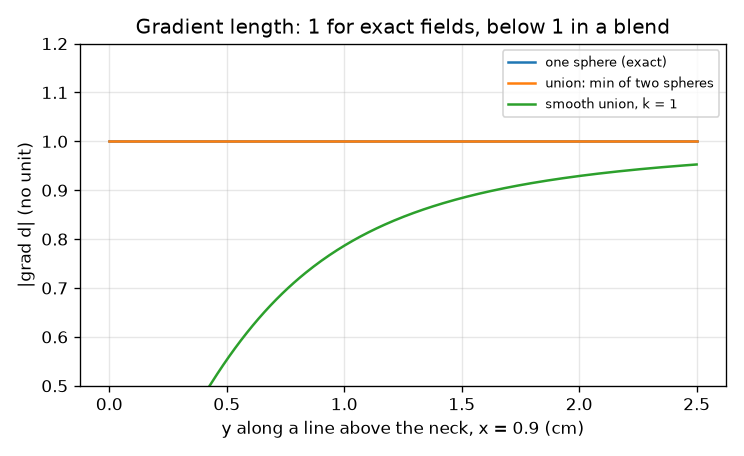
\includegraphics[width=0.85\linewidth]{figures/s03_gradient_norm.png}\\\small Gradient length: 1 for exact fields, below 1 inside a smooth blend.\end{center}

\subsection*{E. Worked example}
For the 300 mL mug (R = 3.852 cm, H = 9 cm, t = 0.5 cm), find the exact volume of the body and of the torus handle, and the mass of the whole mug in a ceramic of density 2.4 g/cm\textasciicircum{}3.
\begin{enumerate}[nosep]
\item Body volume = pi R\textasciicircum{}2 H - pi (R - t)\textasciicircum{}2 (H - t) = 419.5 - 300.0 = 119.49 cm\textasciicircum{}3.
\item Torus volume = 2 pi\textasciicircum{}2 Rh r\textasciicircum{}2 = 2 pi\textasciicircum{}2 * 2.0 * 0.45\textasciicircum{}2 = 7.99 cm\textasciicircum{}3 (full ring; part of it overlaps the wall and the cut-off inner half is removed, so the added volume is smaller).
\item Body mass = 2.4 * 119.49 = 286.8 g.
\item For the handle and its overlap we use the voxel volume of the whole mug (blend radius 0.5 cm): mass of about 301 g.
\item Check: the handle adds about 14 g, which is below the 7.99 cm\textasciicircum{}3 * 2.4 = 19 g of a full torus, as expected since part of the ring is cut away or merges with the wall.
\end{enumerate}
\textbf{Answer.} Body 119.49 cm\textasciicircum{}3 (286.8 g); the whole mug weighs about 301 g with the handle, and the exact torus volume is 7.99 cm\textasciicircum{}3.

\subsection*{F. Questions}
\begin{enumerate}[nosep]
\item \textbf{Conceptual.} Why does the volume error of a voxel count depend on the surface area, and why does it fall about like 1 / N?
\item \textbf{Numerical.} The cavity wall and floor have area 2 pi (R - t)(H - t) + pi (R - t)\textasciicircum{}2. Compute it for R = 3.852, t = 0.5, H = 9 cm and use it to estimate the change in body volume when the wall grows from 0.5 to 0.6 cm (R and H fixed).
\item \textbf{Graph and simulation interpretation.} From the blend-radius results: the empty cavity is 300 mL with no blend, about 294 mL with k = 2 cm, about 166 mL with k = 8 cm and 0 with k = 16 cm. Explain what happens physically and what blend radius you would allow.
\item \textbf{Design and optimisation challenge.} Design: choose the thickest wall in steps of 0.05 cm from 0.30 to 0.80 for a 300 mL mug of height 9 cm that must weigh less than 320 g (ceramic 2.4 g/cm\textasciicircum{}3, blend 0.5 cm). Justify with the numbers and state what the model leaves out.
\end{enumerate}

\section{Real-world mini-project}
\textbf{Design a mug that holds 300 mL and weighs under 320 g.} A ceramics workshop wants a mug of height 9 cm with a handle (ring of radius 2 cm, tube radius 0.45 cm, blend radius 0.5 cm). It must hold 300 mL and weigh less than 320 g in a ceramic of density 2.4 g/cm\textasciicircum{}3. Thick walls are stronger, so the workshop wants the thickest wall in steps of 0.05 cm that still meets the mass limit. For each wall t from 0.30 to 0.80 cm, solve the outer radius for 300 mL with the Session 2 formula, build the mug with \texttt{mug3d} from Session 3, and estimate its mass from the voxel volume with \texttt{mug\_mass}.

\section{The path ahead}
\begin{enumerate}[nosep]
\item \textbf{Session 4: Marching cubes: a 3D mesh and an STL file.} A function that turns the mug field into triangles and writes an STL file.
\item \textbf{Session 5: Repair the field: redistancing.} A routine that turns the field of two crossing half-spaces into a true distance field.
\item \textbf{Session 6: Fewer samples: adaptive octree volume.} A volume estimator that refines only the cells near the surface.
\item \textbf{Session 7: Assembly: a lid that fits.} A lid part positioned on the mug with a fixed clearance.
\item \textbf{Session 8: Sensitivity-driven design.} A Newton iteration on the wall thickness that holds 300 mL.
\end{enumerate}

\section{Answers and hints}

\subsection*{Session 1}
\begin{enumerate}[nosep]
\item \textbf{Conceptual.} Hint: What would a point at the centre of a circle and a point far away both look like if we only used the size of the distance? Solution: A distance with no sign cannot tell inside from outside: a point 1 unit inside and a point 1 unit outside would both read 1. The sign makes the surface exactly the places where the value is zero, and lets us decide inside or outside by checking the sign. It also makes the union simple: take the smaller number.
\item \textbf{Numerical.} Hint: Distance from the origin to (3, 4) first, then subtract the radius. Solution: \textbar{}p - c\textbar{} = sqrt(3\textasciicircum{}2 + 4\textasciicircum{}2) = 5, so d = 5 - 2 = 3 units. Positive, so the point is outside. Sanity check: the nearest point of the circle is 2 units from the centre along the same line, leaving 3 units.
\item \textbf{Graph and simulation interpretation.} Hint: Find where the black curve is below the zero line. Solution: The union is inside for x between -0.954 and 0.954 (circle) and for x between 1.5 and 2.5 (box). Between 0.954 and 1.5 both shape curves are above zero, so the line passes through empty space between the two shapes.
\item \textbf{Design and optimisation challenge.} Hint: The left side of the box is the line x = 1.5. Where does the circle reach along the x axis? Solution: The circle reaches x = r on the x axis, so r = 1.5 makes the two just touch at (1.5, 0): both values are 0 there. With r = 1.6 the point (1.5, 0) has value -0.1 in the circle, so the shapes overlap by 0.1 units. A real part should overlap: with only a touching point the joint has zero thickness and cannot carry load, and round-off could separate the shapes. The trade-off is a slightly bigger part.
\end{enumerate}

\subsection*{Session 2}
\begin{enumerate}[nosep]
\item \textbf{Conceptual.} Hint: Look at what happens to the formula when \textbar{}a - b\textbar{} is larger than k. Solution: When \textbar{}a - b\textbar{} \textgreater{}= k we get h = 0, so smin = min(a, b) exactly: far from the junction nothing changes. Only where the two distances are within k of each other does h become positive and the surface is pulled outward, by at most k / 4 where they are equal.
\item \textbf{Numerical.} Hint: R = t + sqrt(V / (pi (H - t))). Solution: H - t = 9.6 cm; 300 / (pi * 9.6) = 9.947; sqrt = 3.154 cm; R = 0.4 + 3.154 = 3.554 cm. Sanity check: a taller, thinner mug needs a smaller radius than the 3.852 cm of the worked example, as found.
\item \textbf{Graph and simulation interpretation.} Hint: Use k / 4. Solution: k / 4 = 0.5 cm: for a = b = 0 the smooth minimum is -0.5 cm. Away from the crossing, further than k = 2 cm from it, the curves coincide.
\item \textbf{Design and optimisation challenge.} Hint: Use the formula for R, then material = pi R\textasciicircum{}2 H - 300. Solution: For t = 0.4 cm: R = 3.732 cm and material 93.9 cm\textasciicircum{}3. For t = 0.8 cm: R = 4.213 cm and material 201.7 cm\textasciicircum{}3. The thick wall uses more than twice the material (so it is heavier and more expensive) and makes a wider mug, but it is far more robust; the model cannot say how much stronger, so a designer would test samples. A middle value such as 0.5 cm needs 119.5 cm\textasciicircum{}3.
\end{enumerate}

\subsection*{Session 3}
\begin{enumerate}[nosep]
\item \textbf{Conceptual.} Hint: Which voxels can be wrong, and by how much? Solution: Voxels fully inside or fully outside are always judged correctly. Only voxels cut by the surface can be wrong, and each is wrong by at most one voxel volume h\textasciicircum{}3. There are about (surface area) / h\textasciicircum{}2 such voxels, so the error is of order (surface area) * h. Since h is proportional to 1 / N, the error falls like 1 / N. In our measurement the log-log slope is about -1.
\item \textbf{Numerical.} Hint: Multiply the area by the change in thickness; compare with the exact change. Solution: Area = 2 pi * 3.352 * 8.5 + pi * 3.352\textasciicircum{}2 = 179.0 + 35.3 = 214.3 cm\textasciicircum{}2. Estimated change = 214.3 * 0.1 = 21.4 cm\textasciicircum{}3. The exact change is 20.96 cm\textasciicircum{}3, a little smaller, because the cavity area itself shrinks as the wall grows; the estimate is first order in the step. Units: cm\textasciicircum{}2 times cm gives cm\textasciicircum{}3.
\item \textbf{Graph and simulation interpretation.} Hint: Where is the field of the handle within k of the field of the body? Solution: A smooth union adds material wherever the distances to the two shapes differ by less than k, pulling the surface out by up to k / 4. With a large k the region stretches across the whole cavity, which is far from the handle by only a few cm, so the cavity fills. A mug that must hold 300 mL cannot afford a large blend: k = 2 cm already costs about 2 percent of the capacity, so keep k small (the mini-project uses 0.5 cm).
\item \textbf{Design and optimisation challenge.} Hint: Solve R for each t and use mug\_mass; mass grows with t at fixed capacity. Solution: t = 0.50 cm (R = 3.852 cm) weighs about 301 g and passes; t = 0.55 cm (R = 3.912 cm) weighs about 336 g and fails. So the thickest passing wall is 0.50 cm. Left out: strength (a thick wall is stronger but the model cannot say how much), thermal behaviour, a rounded rim, tolerances in the voxel estimate (about 1 percent), and the fact that the 320 g limit would be tested on real pieces.
\end{enumerate}

\section{How to join}
Read \texttt{CONTRIBUTING.md} in the repository, then pick an issue labelled \texttt{good first issue}. Repository: \url{https://github.com/KrunalPanchal1995/opensculpt}

\end{document}
